\documentclass{article}

\usepackage[utf8]{inputenc}
\usepackage[a4paper, total={5in, 8in}]{geometry}
\usepackage{graphicx}
\usepackage[final]{pdfpages}
\usepackage{listings}
\usepackage{amsmath}
\usepackage{subfigure}

\title{\textbf{Cheminfomatics Assignment 2}}
\author{William Juhl}

\date{\textit{December 2023}}

\pagenumbering{arabic}
\begin{document}
%\pagenumbering{gobble}
\thispagestyle{empty}

\maketitle
\newpage
\thispagestyle{empty}

\tableofcontents

\newpage
\section{Introduction}

The goal of this paper is to discuss the implementation of a program that produces chemically correct graph grammar rules for a given set of educt molecules and product molecules. We will first discuss the formal specification of what defines a chemically valid mapping, then we will discuss the implementation of said specification and finally we will discuss the results of the program.

\newpage
\section{Formal definition of a chemically valid mapping}

A chemically valid mapping is defined as a mapping between a subset of the atoms of the educt molecules and a subset of the atoms of the product molecules. It must also also create a singular cycle of even length. This cycle is constructed by XORing the bonds on the educt side with the bonds on the product side while adheering to the following rules: 
\begin{enumerate}
    \item If a bond is present on the educt side but not on the product side, it must be a single bond. This is called a \textit{deletion}.
    \item If a bond is present on the product side but not on the educt side, it must also be a single bond. This is called an \textit{addition}.
    \item If a bond exists between two atoms on both sides the difference in the bonds must not differ by more than one. If the bond on the product side is greater than that on the educt side it is called an \textit{addition} and if the bond on the product side is less than that on the educt side it is called a \textit{deletion}.
    \item For each atom in the cycle it must have exactly one bond that is an addition and one bond that is a deletion.
\end{enumerate}
If all of the above criteria are met, the mapping is considered chemically valid. We can further controll the mapping we are looking for by introducing two parameters, \textit{k} and \textit{c}. Here \textit{c} describes the desired length of the cycle and \textit{k} describes the context of the mapping. The context is defined as the atoms on both sides which do not have changing bonds and with a distance no more than \textit{k} from the cycle. In general \textit{k} controls the level of how generic the mapping is, with smaller \textit{k} making the mapping more generic and bigger \textit{k} making the mapping more specific.

\newpage
\section{Implementation}

In this section we will discuss the implementation of the program. First we will discuss how to generate the morphisms which map the atoms from the educt to the atoms on the product. Then we will discuss how we can use the morphism to construct a new graph by XORing the bonds on the educt side with the bonds on the product side. Then we will expand the morphism to include the desired context based on the parameter \textit{k}. Finally we will discuss how we can detect, construct and validate a potential cycle which indicates a chemically valid mapping. 

\subsection{Morphism Generation}

To lazily generate morphisms we use two generators, \textit{Morphism\_Generator} which employs a helper generator \textit{Combinatorial\_Generator}. The generator picks \textit{c} atoms from the educt and for each unique atom pick the same amount of atoms from the product. This ensures that we have a one-to-one mapping between the atoms from the educt and the atoms from the product and also that we do not have a morphism which maps a Hydrogen atom to a Carbon atom.

\subsubsection{Combinatorial\_Generator}

To pick \textit{n} amount of atoms from a set of atoms we use a bit field where exactly \textit{n} bits are set and a one indicates that the atom is picked. To permute the next combination of \textit{n} atoms we simply permute the bit field. If no more unique combinations can be generated return false, otherwise return true.


\subsubsection{Morhpism\_Generator}

By using the above generator we pick \textit{c} atoms from the educt. For each of the unique atoms from the educt we pick exactly the same amount of atoms from the product. Then constructing a morphism is as simple as mapping the index of the atom from the educt to the index of the atom from the product. We can generate the next morphism by picking the next combination on the product side. If there are no more unique combinations on the product side we pick a new combination on the educt side and start over. Once both sides have no more unique combinations we have generated all possible morphisms. 

\subsubsection{Observations}
From observing and trying different orderings for which atoms are picked initially, we can gain a huge performance boost by mapping Hydrogen atoms last. Because Hydrogen atoms only have a single bond they are not very likely to be part of a cycle. For that reason we can pick them last and thus reduce the number of morphisms we have to generate before finding a valid cycle. To do this we have opted to pick the atoms based on their weight making heavier atoms being picked first for the cycle.

\subsection{Educt XOR Product}
When we have a morphism we can construct a new graph by XORing the bonds on the educt side with the bonds on the product side. This is done by iterating through each atom pair, \textit{left} and \textit{right}, in the morphism and checking for the following:
\begin{enumerate}
    \item If the left atom has a bond to another atom in the morphism and the right atom does \textbf{not} have a bond to another atom in the morphism we have the following two cases:
    \begin{enumerate}
        \item If it is a single bond we add an edge with label REMOVE between the left atom's source and target.
        \item If the bond is a double or a triple bond it is an invalid edge.
    \end{enumerate}
    \item If the left atom does \textbf{not} have a bond to another atom in the morphism and the right atom does have a bond to another atom in the morphism we have the following two cases:
    \begin{enumerate}
        \item If it is a single bond we add an edge with label ADD between the right atom's source and target.
        \item If the bond is a double or a triple bond it is an invalid edge.
    \end{enumerate}
    \item If both the left and the right have a bond to another atom in the morphism we have the following five cases:
    \begin{enumerate}
        \item If the bond on the left is a single bond and the bond on the right is a double add the edge with label ADD.
        \item If the bond on the left is a double bond and the bond on the right is a single bond add the edge with label REMOVE.
        \item if the bond on the left is a double bond and the bond on the right is a triple bond add the edge with label ADD.
        \item if the bond on the left is a triple bond and t he bond on the right is a double bond add the edge with label REMOVE.
        \item Otherwise it is an invalid edge
    \end{enumerate}
\end{enumerate}
The resulting graph is the XORed graph of the educt and the product using the given morphism. If any of the edges are invalid, the morphism is also not chemically valid.

\subsection{Cycle Detection and Construction}

By doing a Depth-First-Search on the XORed graph we can detect cycles by registering when a back edge is found. When a back edge is found we can construct a cycle by following the path from the back edge to the current node. 

\subsection{Cycle validation}

If the above step produces more than a single cycle or if no cycle were detected we discard this morphism. Otherwise we can validate the cycle by checking if the cycle is of even length and if the cycle contains exactly one addition and one deletion for each atom in the cycle.

\subsection{Context Expansion}

To add the context defined by the parameter \textit{k} we simply expand the morphism to include all atoms within \textit{k} bonds of the cycle which adhere to both of the two following conditions:
\begin{enumerate}
    \item The bond must be the same on the educt side as on the product side
    \item The atom must be connected to the morphism on both sides.
\end{enumerate}
This ensures that we only expand the morphism to include atoms which can reach the cycle within \textit{k} bonds and which share the same bond strength on the educt and the product side.

\newpage
\section{Results}
We will now compute a series of tests to see how the program performs. I am running the program inside a Docker container with the Rosetta translation layer on my Macbook Pro running a 10 core M1 Pro processor with access to 8 GB of RAM out of a total of 16 GB of RAM. In the below table  
\begin{table}[h]
    \centering
    \begin{tabular}{ll|ccccc}\\
        Educts & Products & $k$ & $c$ & $n$ & $t$ & $s$\\\hline
        C=C, C=C & C1CCC1 & 0 & 4 & 2 & 10 & 0.250s \\
        C=C, C=C & C1CCC1 & 1 & 4 & 2 & 10 & 0.255s \\
        O, Cl, CC(=O)OCC & Cl, OCC, CC(=O)O & 0 & 6 & 3 & 10 & 0.804s \\
        O, Cl, CC(=O)OCC & Cl, OCC, CC(=O)O & 1 & 6 & 3 & 10 & 0.804s \\
        O, Cl, CC(=O)OCC & Cl, OCC, CC(=O)O & 2 & 6 & 3 & 10 & 0.811s \\
        C1C(O)CC(O)C(O)C1 & C=CO, C=CO, C=CO  & 0 & 6 & 4 & 10 & 0.437s \\
        C1C(O)CC(O)C(O)C1 & C=CO, C=CO, C=CO  & 1 & 6 & 6 & 10 & 0.455s \\
        CC=CC=CC, OC1C=CC=CC=1 & C=CC=CC=C, OC(=C)C=CC=C & 0 & 6 & 4 & 10 & 4.169s \\
        CC=CC=CC, OC1C=CC=CC=1 & C=CC=CC=C, OC(=C)C=CC=C & 1 & 6 & 6 & 10 & 4.163s \\
        CC=CC=CC, OC1C=CC=CC=1 & C=CC=CC=C, OC(=C)C=CC=C & 2 & 6 & 7 & 10 & 4.146s \\
        CC, OC1C=CC=CC=1 & C=C, OC(=C)C=CC=C & 0 & 6 & 4 & 10 & 3.266s \\
        CC, OC1C=CC=CC=1 & C=C, OC(=C)C=CC=C & 1 & 6 & 4 & 10 & 3.264s \\
        CC, OC1C=CC=CC=1 & C=C, OC(=C)C=CC=C & 2 & 6 & 4 & 10 & 3.290s \\
        OP(=O)(O)OP(=O)(O)O, O & O=P(O)(O)O, O=P(O)(O)O  & 0 & 4 & 1 & 10 & 0.322s \\
        OP(=O)(O)OP(=O)(O)O, O & O=P(O)(O)O, O=P(O)(O)O  & 1 & 4 & 1 & 10 & 0.317s \\
        OP(=O)(O)OP(=O)(O)O, O & O=P(O)(O)O, O=P(O)(O)O  & 0 & 6 & 1 & 10 & 0.399s \\
        OP(=O)(O)OP(=O)(O)O, O & O=P(O)(O)O, O=P(O)(O)O  & 1 & 6 & 1 & 10 & 0.397s \\
        C\#N, C\#N & N=CC\#N & 0 & 4 & 1 & 2 & 0.254s \\
        C\#N, C\#N & N=CC\#N & 1 & 4 & 1 & 2 & 0.270s \\
    \end{tabular}
    \caption{
        \textit{k} is the context, \textit{c} is the cycle length, \textit{n} is the number of unique rules found and \textit{t} is  the number of valid morphisms generated. The last column is the \textit{real} time it took to generate the rules. The time is measured in seconds.
    }
    
\end{table}
\newpage
\section{Example}

To illustrate how a difference in context will affect the derivations, we have constructed the following example.

From the above table, derive the rules with cycle length of 6 from the third row. We have however removed the Chlorid from the educt and the product side. Then by adding to the subset only the educts and applying the generated rules once will result in the below figure. We will use context arguments of $0$ and $1$ and depict them below.

As we can observe (a) contains a bigger hypergraph than that in (b).

\begin{figure}[h!]
    \centering
    \caption{Hypergraphs from running a derivation once with the generated rules.}
    \subfigure[Context k = 0]{\includegraphics[trim = 1.5cm 12.6cm 1.5cm 2.3cm, clip,page=3, width=0.8\textwidth]{example_k0.pdf}}
    \newline
    \subfigure[Context k = 1]{\includegraphics[trim = 1.5cm 12cm 1.5cm 2.4cm, clip,page=3, width=0.8\textwidth]{example_k1.pdf}}
\end{figure}

\newpage
\section{Improvements}
The main improvement that can be done is to speed up finding valid morphisms resulting in unique rules. Currently we are generating all possible morphisms without checking for symmetry. My hypothesis is that many of the morphisms we generate result in the exact same rules. This can be seen by the number of discarded rules from the table above. By pruning the morphisms from the same cycle which result in an identical rule we can get a more diverse set of rules.



\end{document} 

